%%%%%%%%%%%%%%%%%%%%%%%%%%%%%%%%%%%%%%%%
%% MCM/ICM LaTeX Template %%
%% 2021 MCM/ICM           %%
%%%%%%%%%%%%%%%%%%%%%%%%%%%%%%%%%%%%%%%%
\documentclass[12pt]{article}
\usepackage{geometry}
\geometry{left=1in,right=0.75in,top=1in,bottom=1in}

%%%%%%%%%%%%%%%%%%%%%%%%%%%%%%%%%%%%%%%%
% Replace ABCDEF in the next line with your chosen problem
% and replace 1111111 with your Team Control Number
\newcommand{\Problem}{MCM Problem A}
\newcommand{\Team}{2125756}
%%%%%%%%%%%%%%%%%%%%%%%%%%%%%%%%%%%%%%%%

\usepackage{newtxtext}
\usepackage{amsmath,amssymb,amsthm}
\usepackage{newtxmath} % must come after amsXXX

\usepackage[pdftex]{graphicx}
\usepackage{xcolor}
\usepackage{fancyhdr}
\usepackage{lipsum}
\usepackage{multicol,caption}
\usepackage{subcaption}

\usepackage{footnote}
\usepackage{float}
\restylefloat{table}
\usepackage{adjustbox}

%\usepackage{syntonly}
%\syntaxonly


\usepackage[utf8]{inputenc}
\usepackage[english]{babel}

\usepackage[
backend=biber,
style=chem-angew,
sorting=ynt]{biblatex}
\addbibresource{masterbib.bib}

\lhead{Team \Team}
\rhead{}
\cfoot{}

\newtheorem{theorem}{Theorem}
\newtheorem{corollary}[theorem]{Corollary}
\newtheorem{lemma}[theorem]{Lemma}
\newtheorem{definition}{Definition}

%%%%%%%%%%%%%%%%%%%%%%%%%%%%%%%%

\newenvironment{ColumnFigure}
{\par\medskip\noindent\minipage{\linewidth}}
{\endminipage\par\medskip}

\begin{document}
\graphicspath{{.}}  % Place your graphic files in the same directory as your main document
\DeclareGraphicsExtensions{.pdf, .jpg, .tif, .png}
\thispagestyle{empty}
\vspace*{-16ex}
\centerline{\begin{tabular}{*3{c}}
	\parbox[t]{0.3\linewidth}{\begin{center}\textbf{Problem Chosen}\\ \Large \textcolor{red}{\Problem}\end{center}}
	& \parbox[t]{0.3\linewidth}{\begin{center}\textbf{2021\\ MCM/ICM\\ Summary Sheet}\end{center}}
	& \parbox[t]{0.3\linewidth}{\begin{center}\textbf{Team Control Number}\\ \Large \textcolor{red}{\Team}\end{center}}	\\
	\hline
\end{tabular}}
%%%%%%%%%%% Begin Summary %%%%%%%%%%%
% Enter your summary here replacing the (red) text
% Replace the text from here ...
\begin{center}
\textcolor{red}{%
\lipsum[1]
}
\end{center}
% to here
%%%%%%%%%%% End Summary %%%%%%%%%%%

%%%%%%%%%%%%%%%%%%%%%%%%%%%%%%
\clearpage
\begin{multicols}{2}
\tableofcontents
\listoftables
\newpage
\pagestyle{fancy}
% Uncomment the next line to generate a Table of Contents
%\tableofcontents 
\newpage
\setcounter{page}{1}
\rhead{Page \thepage\ }
%%%%%%%%%%%%%%%%%%%%%%%%%%%%%%


	
%\section{Pre-planning analysis}
%- 
	
\section{Introduction}

Decomposition by fungal and microbial communities is second only to photosynthesis in driving carbon cycling in the Earth's ecological communities \cite{McGuire2010}. While this significance is rarely understated, inner mechanisms and interactions within decomposition communities have been poory understood and treated as a 'black box' in the past by scientists studying ecosystem processes \cite{Andren1999}.

Fungi are made up of hyphae: long winding filaments enmeshed together to form a thick mat of mycelium. At the frontline of battle, hyphal tips are extending forward and branching to cover new area at a velocity dictated by the hyphal extension rate, and concurrently other hyphae are dying off or merging together \cite{Edelstein1982}. Like machinery, each fungus has ideal operating conditions. Fungi native to dry or arid biomes will grow efficiently in a moisture-lacking environment when other fungi will falter. Maynard et al. (2019) defines these operating conditions by assigning temperature and moisture niche-widths to 37 studied species of fungi \cite{Maynard2019}.

\subsection{Competition}
When fungi come into contact with each other, competitive interactions are most often observed. Tactics studied in Boddy, L. (2000) include deploying diffusable toxins, obtaining nutrients parasitically, destruction of hyphae by intentional interference, and establishing wall-like barracades to thwart attackers \cite{Boddy2000}. Most researchers, including Maynard et al. (2019) construct a competitive ranking scale based on experimental observations to encapsulate the ramifications of these complex interactions \cite{Maynard2019}.

Under a constant temperature regime, previous research concludes that dominant fast-growing suppress other species which negatively impacts the overall community's efficiency. However fluctuating environmental conditions change the outcome and promote complementary growth \cite{Toljander2006}. An explanation for this is presented by Lustenhouwer et al. (2020) suggesting a spectrum between slow-growing, stress-tolerant fungi operating in a wider environmental range than fast-growing, highly competitive fungi \cite{Lustenhouwer2020}. 

\subsection{Substrates}
Determining which fungi are present in a community depends on the organic material, or 'substrate', being broken down. In the case of fungal-mediated wood decomposition, the substrate is made up of lignocellulose polysaccarides, and the fungi involved are equipped with specialized enzymes capable of splitting linkages in the polymers to harvest usable carbohydrates. Long-term wood decomposition follows a well-studied three-phase process: the first phase is dominated by fast and opportunistic fungus claiming easily-consumable soluble sugars, followed in the second phase by consistent and dependable decomposers that degrade the holocellulose constituting 65\%-85\% of the material \cite{Segato2014}. Slow and highly specialized fungi trail behind in the third phase to clean up rigid lignin polymers (15\%-35\%) with powerful oxidative enzymes \cite{Moorhead2006}. While phase progression is an important agent governing community changes on the long-term scale, this paper will focus on only the middle phase of cellulose decomposition and will not conider lignin decomposition. \cite{Lustenhouwer2020}.

\subsection{Growth Model}
An important step in modeling fungal communities is acknowledging separation between the growth rate and the decomposition rate of the fungus, which are influenced by different factors. Fungal growth models typically focus on the increase in overall biomass due to hyphal extension. Fungi with a greater density of hyphal tips per unit volume will grow and accrue biomass faster, as hyphae only grow from their tips. New tips are are created when hyphae branch off, while others die or fuse together via anasmotosis. Edelstein (1982) models these dynamics with the following:

\begin{equation} \label{eq:1}
\frac{\partial \rho}{\partial t} = n\nu - d
\end{equation}
\begin{equation} \label{eq:2}
\frac{\partial n}{\partial t} = -\frac{\partial n\nu}{\partial x} + \sigma
\end{equation}

Where \textbf{************} These equations will operate standing alone, without any other influences by enzymes or growth limitations. This allows many models to treat it as a baseplate to expand upon. Edelstein (1983) and Davidson et al. (1997) do this by considering concentrations of nutrients inside the fungi and outside in the surrounding substrate \cite{Edelstein1983, Davidson2012}. Our model will likewise follow in eliminating the assumption that fungi grow over an unlimited nutrient supply. A more contemporary approach by Du et al. (2019) describes the growth of a fungus with a 3-dimensional reaction-diffusion equation based on microscopic growth mechanisms, also focusing on tip density and extension rate but with an added term to identify the proportion of tips which are actively growing \cite{Du2019}.

\subsection{Environmental Influence on Hyphal Tip Extension ($\nu$)}
Environmental impacts are introduced to the decomposition model through $\nu$, the hyphal tip elongation rate. The mechanism of elongation is relatively unknown; as described in Gervais et al. (1999), "cell turgor pressure corresponds to an overpressure which allows the cell morphology, elongation, division and hence the biomass evolution" \cite{Gervais1999, Steinberg2007}. In fungi, cell turgor comes from diffusion of water dictated by the water potential\footnote{Water potential ($\psi$) describes the content of availability of moisture surrounding a fungi as dictated by the soil composition.} gradients rather active transport within the cell, making it very environmentally dependent \cite{Gervais1999}. This fact justifies determining $\nu$ based on environmental factors on fungal decomposition rates by varying $\nu$ outside of baselines for given species in set locations in our model. Experimental data from Maynard et al. (2019) shows the relationship between $\nu$ and the environmental parameters of water potential ($\psi$) and temperature ($T$) \cite{Maynard2019}.

%\begin{figure*}
%	\centering
%	%\vspace*{-2ex}
%	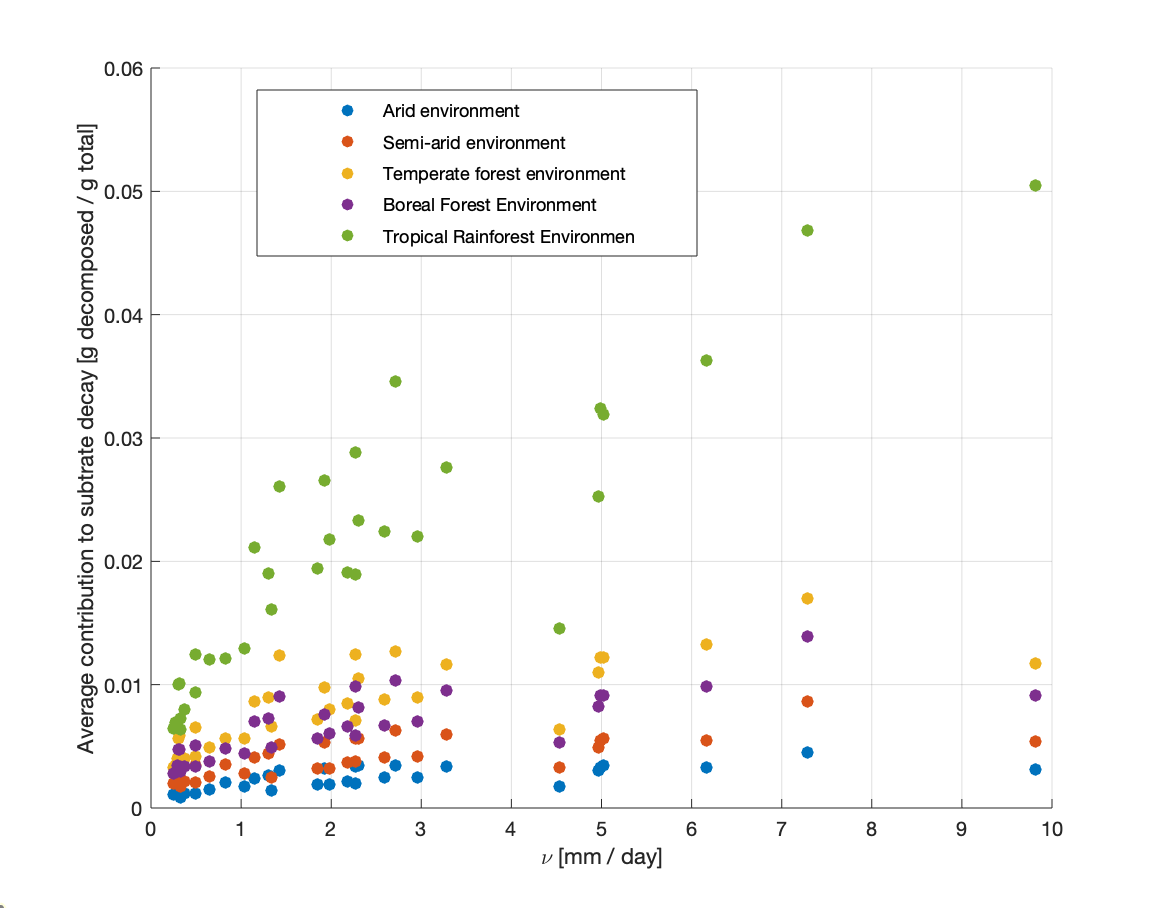
\includegraphics[width=0.7\linewidth]{avg_contr_nu_environment.png}
%	\caption[Fig 1.]{Example optimized flight plan, ran with drone fleet size of 5, starting configuration 1, 5 allowed movements, and $\gamma$ = 2}
%	\label{Fig 1.}
%\end{figure*}
\subsection{Decomposition kinetics}
Moore et al. (2015), Edelstein (1983), Moorhead et al. (2006), Parnas (1974), and Schimel et al. (2003) describe the decomposition of a certain substrate by a microbial decomposer as a function of the substrate's concentration with the Michaelis–Menton equation \cite{Moore2015, Edelstein1983, Moorhead2006, Parnas1975, Schimel2003}. Thus, decompostion of carbon in a substrate is described by the following equation.

\begin{equation} \label{eq:3}
\frac{dC}{dt} = \frac{KBC}{K_{e}+C}
\end{equation}

Where \textbf{******************}. Schimel et al. (2003) and Moorhead et al. (2006) assert that decomposition levels off at a maximum rate proportional to the concentration of enzymes acting on it \cite{Schimel2003, Moorhead2006}. To determine this enzyme concentration, we will make the assumption that enzyme concentration is proportional to the concentration of biomass in our system represented by $r$ multiplied by two environmental limiting factors in $K=rS_{M}S_{T}$ \cite{Schimel2003}. This environmental factors are discussed at greater length in \textbf{section that they're discussed}

\subsection{Enzyme interactions}

Enzymes produced by fungi are expelled into the surrounding substrate to autonomously break down macromolecules. Relative enzyme concentrations can be quantified by the production rates of each enzyme by a fungus. Production of enzymes is a metabolically taxing process, therefore fungi that produce enzymes which return much more usable energy and C than was put into making the enzyme, a high "return on investment", will be able to synthesize even more enzymes and grow rapidly \cite{Schimel2003}. Lustenhouwer et al (2020) strengthens this theory by showing through statistical analysis of 1582 various fungal isolats that fungi containing larger proportions of enzymes like acid phosphatase, which are associated with slow lignin decomposition, are demonstrated to strongly correlate with slower decomposition rates \cite{Lustenhouwer2020}. Lignin exemplifies a low return on investment, requiring powerful enzymes and greater energy input per unit C than holocellulose. But it's ultimately the fungi that have a subset of enzymes that best match their surrounding substrate which successfully grow and establish a niche. As an example, in a substrate of 70\%+ lignin, the slower growing fungi with lignin enzymes normally at a disadvantage will win out over other fungi competing for a fraction of available holocellulose.

Communities with similar fungi of similar enzymatic makeup often see a few dominant species overwhelm the rest through competition for similar resources in the substrate, but communities of fungi with greatly differing enzymes will instead form distinct niches that partition different resources in which they are seperately able to grow. In these conditions, one dominant species faces difficulty in wiping out competitors who are individually masters of their own substrates. This effect is known as niche complementarity \cite{Toljander2006}. Research by Toljander et al. (2006) contends that environmental fluctuations further robustify a diverse community as faster growing highly competitive fungi are hindered by conditions that lapse out of their moisture and temperature niche, and slower growing stress-tolerant fungi benefit from decreased pressure by competitors. The resulting dampened and stable diverse community will decompose the most efficiently across a range of conditions \cite{Toljander2006}.

\section{Model Formulation}


\subsection{Growth Model}
In the review of various fungal growth models described in Lin et al. (2016), a specific method of modeling branching and hyphal death was found to match experimental observations in the widest variety of settings. Based on these results, for $\sigma$ and $d$ in (\ref{eq:1}) and (\ref{eq:2}) we will choose to implement the following relationships, comprising dichotomous branching, tip-hypha anastomosis, and hyphal death (or YHD). 
\begin{equation} 
\sigma = \alpha_{1}*n - \mu n \rho
\end{equation}

\begin{equation}
d = \gamma_{1}\rho
\end{equation}

Enzymes conducting decomposition make up a fraction of the total biomass, and the total biomass changes according to the growth rate. The total biomass $B$ defined in (\ref{eq:8}) multiplies by maximum rate of the Michaelis-Menion equation (\ref{eq:3}) to couple growth rate with decomposition rate. 

\begin{equation} \label {eq:8}
B = \int_{all x}\rho dx
\end{equation}

The rate of decomposition of carbon will then be dynamically effected by the growth of the fungus contrary to the typical assumption of a static $B$ as described by Schimel et al. (2003) \cite{Schimel2003}. Our formulation of $K$ which accounts for the proportion of biomass in the fungal growth containing the necessary enzyme for the carbon decomposition will change to account for this. 
\begin{equation} \label {eq}
K = r*S_{M}*S_{T}*0.04*G
\end{equation}
Where $r$ is a dimensionless parameter representing the relative abundance of one enzyme out of the total enzyme biomass of that specific fungus. The multiplication by $0.02$ is a generalization that for any given species of fungus, 2\% of the biomass will be relevant enzymes \cite{Moorhead2006}. $G$ is an empirically derived rate constant relating the mass of relevant enzymes to the maximum rate of the decomposition.

Limited carbon availability will also impact a fungi's growth rate. To account for this, we include a term multiplying $\nu$ that can be interpreted as the available carbon for the fungi to consume for growth. The first equation in the growth model then becomes
\begin{equation} \label{eq:10}
\frac{\partial \rho}{\partial t} = (1-LCI)*(10^{9})*C*n*\nu - d
\end{equation}
Where $LCI$ is the lignocellulose index\footnote{The lignocellulose index describes the ratio of non-hydrolysable lignin to hydrolysable holocellulose in litter} of a certain material and $(1-LCI)$ is then the proportion of the substrate carbon stored in holocellulose. Multiplying by $(1*10^{9}$ is approximation to convert grams of carbon to hyphae length in mm. [citation needed for g to mm] An investigation of the effects of including the carbon term in the growth model are addressed in a later section. \\

So our coupled growth and decomposition models can be summarized by equations (\ref{eq:2}), (\ref{eq:3}), (\ref{eq:8}), and (\ref{eq:10}).

\subsection{Defining Representative Enzymes}

Maynard et al. (2019) collected data for 8 relevant enzymes and utilized a standard clustering approach to create a subset of four enzymes which best represented the effects by the fungi's enzymatic makeup on competitive interactions \cite{Maynard2019}. Our model utilizes this open-source data by normalizing the production rates of each enzyme and calculating their relative abundance as a fraction of the total enzyme biomass for that specific fungus. Interactions caused by differing rates of decomposition among different enzymes in varying environmental conditions is then represented in our model by taking the weighted sum of all contributions to the decomposition rate from any one of four enzymes in a given fungi species, represented in the following equation
\begin{equation} \label{eq}
\frac{dC_{1}}{dt} = c_{1,a}\frac{de_{1,a}}{dt} + c_{1,b}\frac{de_{1,d}}{dt} + c_{1,c}\frac{de_{1,c}}{dt} + c_{1,d}\frac{de_{1,d}}{dt}
\end{equation}
Where $c_{1,a}$ is a enzyme breakdown efficiency coefficient for the fungal species $1$ and enzyme $a$. Here the rate $\frac{dC_{1}}{dt}$ is representative of the rate of decay of the substrate by the fungi species $1$. Breakdown efficiencies $c_{1,a}$ for each enzyme were derived from correlation coefficients drawn from experimentally observed data in Lustenhouwer et al. (2020) \cite{Lustenhouwer2020}. 

The total decomposition rate is then given by the sum of all rates over the various species of fungi.
\begin{equation} \label{eq}
\frac{dC_{tot}}{dt} = \sum_{i=1}^{n}\frac{dC_{i}}{dt}
\end{equation}
Where $n$ is the total number of fungi being simulated. \textbf{address the fact that all the 35 fungi will be growing/decomposing together at the same time}

\subsection{Estimating $\nu$ For Various Environments}

When considering a sampling of decomposition rates in various environment types, we must determine how to estimate temperate and water potentials that ground fungi would experience. In the case of determining $\nu$, this requires finding projected temperature and water potential.

Amongst existing biome classification models, Whitaker's scheme \cite{Whittaker1970} is notably simple, providing a layout of biomes based on mean annual temperature and mean annual precipitation. However, modern classification of biomes has drifted away from using these traits as definitive biome identifiers \cite{Mucina2018}. These traits alone do not define all features of concern to fungal growth, such as soil composition for example. In addition, by Whitaker's scheme, we find that a given biome can have a wide range of average annual temperatures (such as arid desserts ranging from about -10 to 30 $^{\circ}C$) \cite{Whittaker1970}. We can sample a range of temperature and moisture values to output various $\nu$ and then select certain regions to profile in order to gauge potential environments where fungi can decompose and interact.
%We will sample within the temperature range of Whitaker's scheme: $-15^{\circ}$ to $30^{\circ}$ C of mean annual temperature.

The following are the specific environments selected to represent various biomes:

\end{multicols}

\begin{savenotes}
	\begin{table}[H]
		\begin{center}
			\begin{tabular}{|c c|} 
				\hline
				Biome & Specific Environment Selected \\ [0.5ex] 
				\hline\hline
				Dessert (Arid) & Sonoran Desert, USA \\ 
				\hline
				Grasslands/shrublands & (Semi-Arid), central Argentina\\
				\hline
				Temperate Forest & Sal Forests, central Himalayas\\
				\hline
				Boreal Forest (Arboreal) & Pine Forests, central Himalayas\\
				\hline
				Tropical Rain Forest & Tropical Forests, Barro Colorado Island, Panama \\
				\hline
			\end{tabular}
			\vspace*{-3ex}
			\captionof{table}{Specific Environments}\label{table1}
		\end{center}
	\end{table}
\end{savenotes}

Although water potentials can be approximated based on predictive models, the measure is best found experimentally from soil samples \cite{Abkenar2019}. Single water potential and annual temperature values were selected from ranges of values experimentally determined by a variety of field studies on these environments (see: Table 2). This decision was made since we're aiming to compare discrete environmental conditions rather than create a complete span of environmental conditions.

%% ACTUAL TABLE
\begin{table}[H]
	\begin{center}
		\begin{tabular}{|c c c|} 
			\hline
			Biome/ Environment & Temperature [$^{\circ}C$] & Water Potential [MPA]\\ [0.5ex] 
			\hline\hline
			Dessert (Arid) & 15 & -4.5 \\ 
			\hline
			Grasslands/shrublands (Semi-Arid) &15.3 & -3.2\\
			\hline
			Temperate Forest & 12.49 & -1.09 \\
			\hline
			Boreal Forest (Arboreal)& 12.49 &  -1.51 \\
			\hline
			Tropical Rain Forest & 27.5 & -0.79 \\
			\hline
		\end{tabular}
		\vspace*{-3ex}
		\captionof{table}{Temperature \& Water Potentials}\label{table2}
	\end{center}
\end{table}

Note that these are not wholly representative configurations, but rather examples to provide insight into how fungal species with specific traits may respond in discrete and distinct conditions likely to exist. We can then find $\nu$ using experimental data from Maynard et al 2019 \cite{Maynard2019}.\textbf{talk about continuous data technique thingy in the extra methods info sheet}

\begin{multicols}{2}	
\subsection{Other Responses to Temperature and Water Potential}

Our growth model takes into account temperature (T) and water potential ($\psi$) in two more parameters: the soil temperature coefficient ($S_T$) and the soil temperature coefficient ($S_M$). Moorhead et al. (1991) provides a simple relationship between $S_T$ and T using the rate of increase (Q):
\begin{equation}
\log_{10}(S_T) = \frac{T-25}{10}\log_{10}(Q)
\end{equation}
Although this equation does not take into account specific fungal response to temperature change, more recent evidence supports that this relationship is not direct, with most of the direct impact coming from moisture \cite{Petraglia2018}. As the ratio of rates of decomposition given a temperature change, Q as a parameter should represent the effective output of various mechanisms influenced by temperature rather than focusing on specific mechanisms. However, for the sake of simplicity, Q has been set standard constant to a value of 2.5 \cite{Moorhead1991}.

Water potential also relates to a constant, $S_M$, in a simple equation described in Moorhead et al. (1991) using $\alpha_2$ and $\lambda$:
\begin{equation}
S_M = \alpha_2 -\lambda \log_{10}(-\psi)
\end{equation}

These two parameters help calculate the maximum growth rate by the relationship:
\begin{equation}
\beta = S_T S_M r
\end{equation}
\textbf{why is this $\beta$ and not K?} 

\subsection{Assumptions}

Further assumptions made in the formulation of our model that have not yet been discussed are largely simplifications that are not relevant to any significant or interesting discussion. An itemized list of these assumptions is provided below.
\subsubsection{Growth}
\begin{itemize}
	%\item Growth occurs in a 1-dimensional space *we should mention this in the formulation
	\item Neglecting effects from direct interactions between fungi
	\item Neglecting effects from N limitation
	\item Litter is not added to or removed from the carbon pool by forces external of the fungi
	\item LCI is xxx and remains constant over time
	\item Dynamics regarding the rate of nutrient absorption and transport of metabolites within the
	mycelium are ignored or simplified *more specific
	\item Ignoring other growth traits: LIST
	%\item Substrate use efficiency (SUE) is 1 *should be in the model formulation
	\item Hyphal death rate $\gamma_{1}$ remains constant regardless of environmental fluctuations
	\item 100\% of living hyphal tips are active
	\item No biomass created by a fungus will be geometrically isolated from the substrate
	\item Neglecting effects due to spacial limitations
	%\item decomposition coefficients are representative of those families of enzymes
\end{itemize}
\subsubsection{Decomposition Kinetics}
\begin{itemize}
	\item Neglecting effects due to enzymes not included in the model
	\item Production of enzymes increases proportionally with biomass
	\item For any species of fungus, 2\% of the biomass will be relevant enzymes
	\item Relative proportions of enzymes will stay constant regardless of environmental fluctuations
	\item Neglecting effects on decomposition rate due to changing metabolic rate of the fungi
\end{itemize}
\subsubsection{Temperature/Moisture effects}
\begin{itemize}
	\item Turgor is a function of water potential
	\item Fungal decomposition occurs in surface soil (0-30 cm)
	\item Experimental data for water potentials in specific biomes/environments are representative of the conditions of those environments
	\item Rate of increase of temperature $Q$ remains constant regardless of environmental fluctuations
\end{itemize}

\section{Parameter selection and representative result}
We created a representative run of the coupled growth and decomposition model to select realistic values for the parameterts, with some values found by consulting literature. An overview of the parameter selection for this representative run can be seen in Table \ref{table3}, however several parameters are worth some discussion.
 
\subsection{Growth model parameters}
Two main parameters were studied for their effect on the growth model's result: the branching rate and the hyphal death rate. These parameters were not agreed upon in literature so values were selected from a pool of possible valus depending on their effect on the model to converge on the most likely realistic output. 

Most results of the growth model were comprised of traveling wave solutions, converging to a uniform distribution in both space and time. This can be thought of as a convergence to the maximum growth of the fungus into its total space. The branching rate ($\alpha_{1}$) was found to increase the hyphal density in the end behavior of the solution, with the ending density increasing as $\alpha_{1}$ increases. The hyphal death rate ($\gamma_{1}$) was found to increase the oscillations in time and larger $\gamma_{1}$ values would increase the oscillations and the time to reach a given end-behavior. Many papers (Edelstein (1982), Lin et al. (2016), Schnepf et al. (2007), Du et al. (2019)) discussing the values of these parameters were concerned more with short-term dynamics in perfectly ideal conditions \cite{Edelstein1982, Lin2016, Schnepf2008, Du2019}. The purposes of this paper is the assess the longterm decomposition rates under variable conditions, so parameters that could predict long-term behavior, comparable to long term decomposition dynamics described in Moorhead et al. (2000), Moorhead et al. (2006), and Moorhead et al. (1991) were selected \cite{Moorhead1991, Moorhead2000, Moorhead2006}.

%\end{multicols}
%\begin{center}
%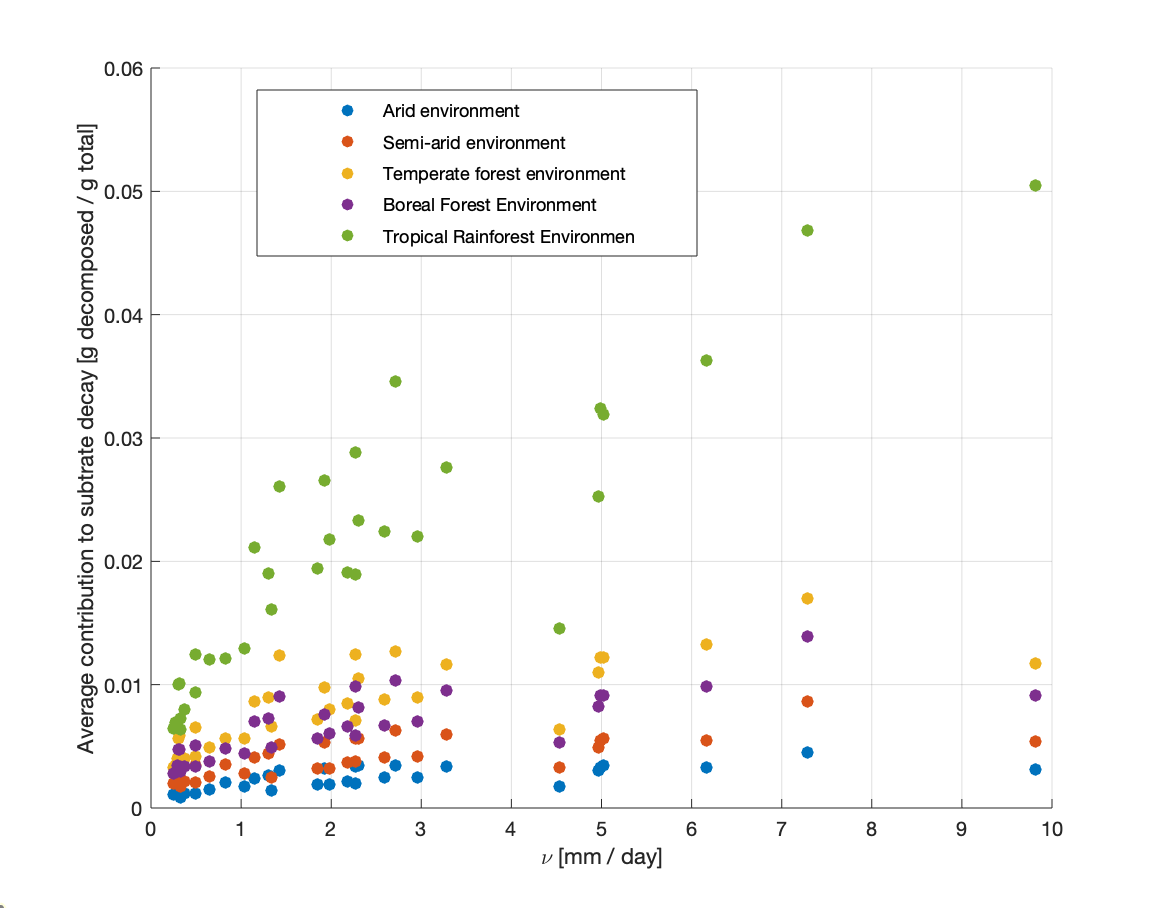
\includegraphics[width=\linewidth]{avg_contr_nu_environment.png}
%\captionof{figure}{Figure caption}
%\label{Fig 2.}
%\end{center}
%\begin{multicols}{2}

\subsection{Decomposition parameters}
The value for $G$ represents a rate constant relating the concentration of relevant enzymes to the maximum rate of carbon decomposition. Formulation for $S_{M}$ and $S_{T}$ come from Moorhead et al. (1991) which uses a simpler equation to describe the reaction dynamics for decomposition of carbon \cite{Moorhead1991}. Our model adds complexity to this so we based this parameter on agreement with other more similar models and experimental data. The most important conclusion drawn for $G$ was in selecting a timescale of decomposition to be comparable with that of Lustenhouwer et al. (2019) \cite{Lustenhouwer2020}.

\end{multicols}
\begin{figure}[H]
	\begin{subfigure}[t]{0.5\textwidth}
		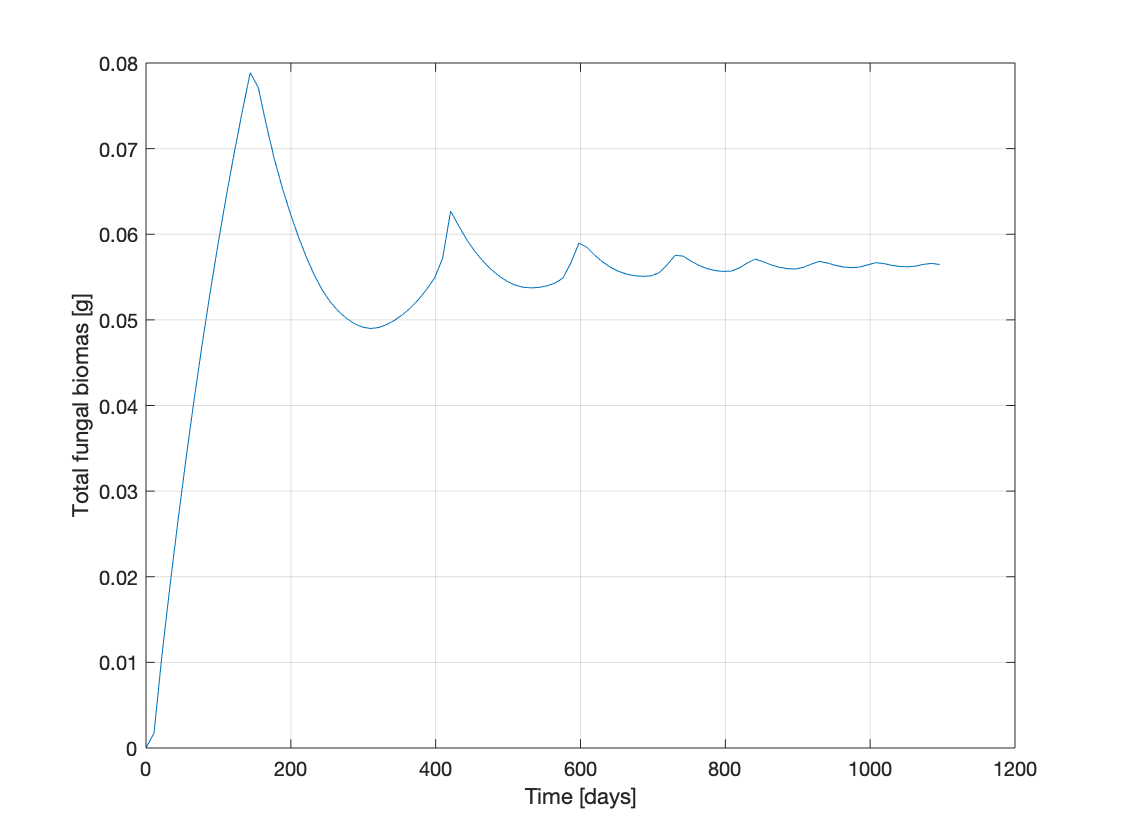
\includegraphics[width=\textwidth]{biomass_growth_no_Cterm.png}
		\caption{Modello compartimentale mammellare (o mammillare).}
		\label{fig-a}
	\end{subfigure}\hfill
	\begin{subfigure}[t]{0.5\textwidth}
		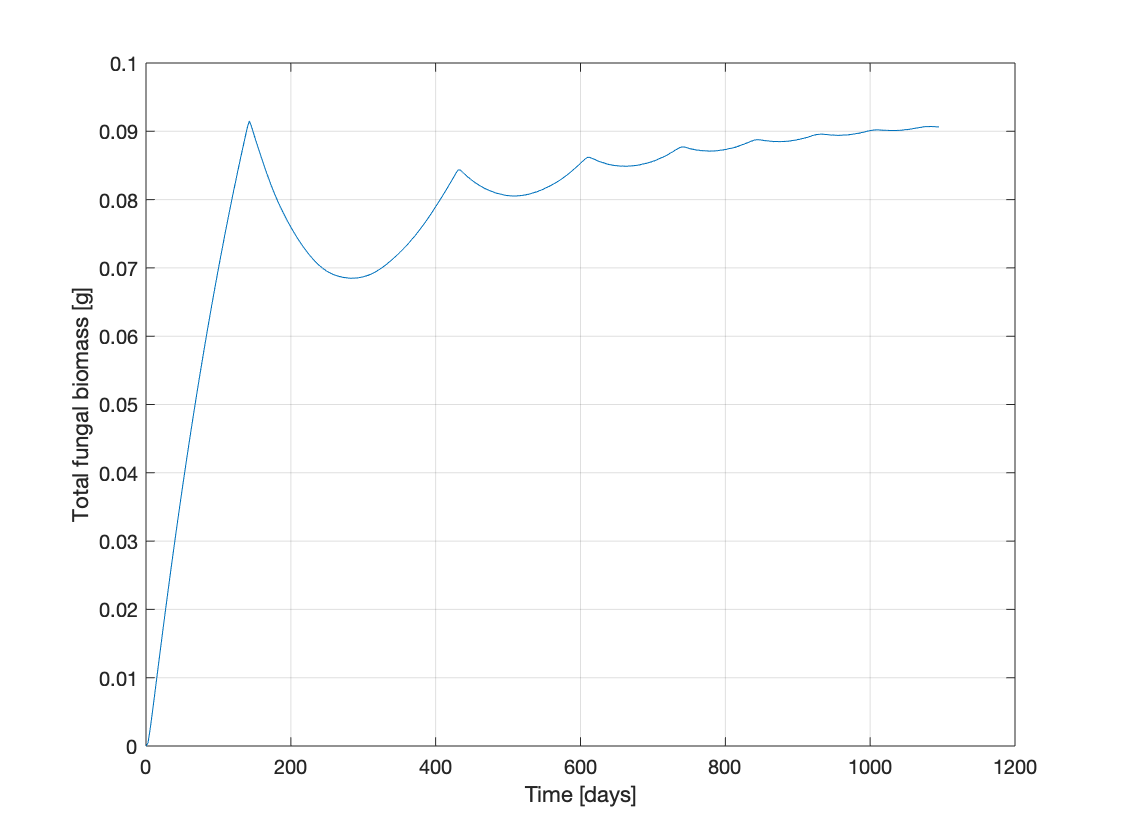
\includegraphics[width=\textwidth]{biomass_growth_Cterm.png}
		\caption{Modello compartimentale catenario.}
		\label{fig-b}
	\end{subfigure}
	\caption{Principali topologie dei modelli compartimentali.} 
	\label{fig:main}
\end{figure}
\begin{multicols}{2}

%\end{multicols}
%\begin{center}
%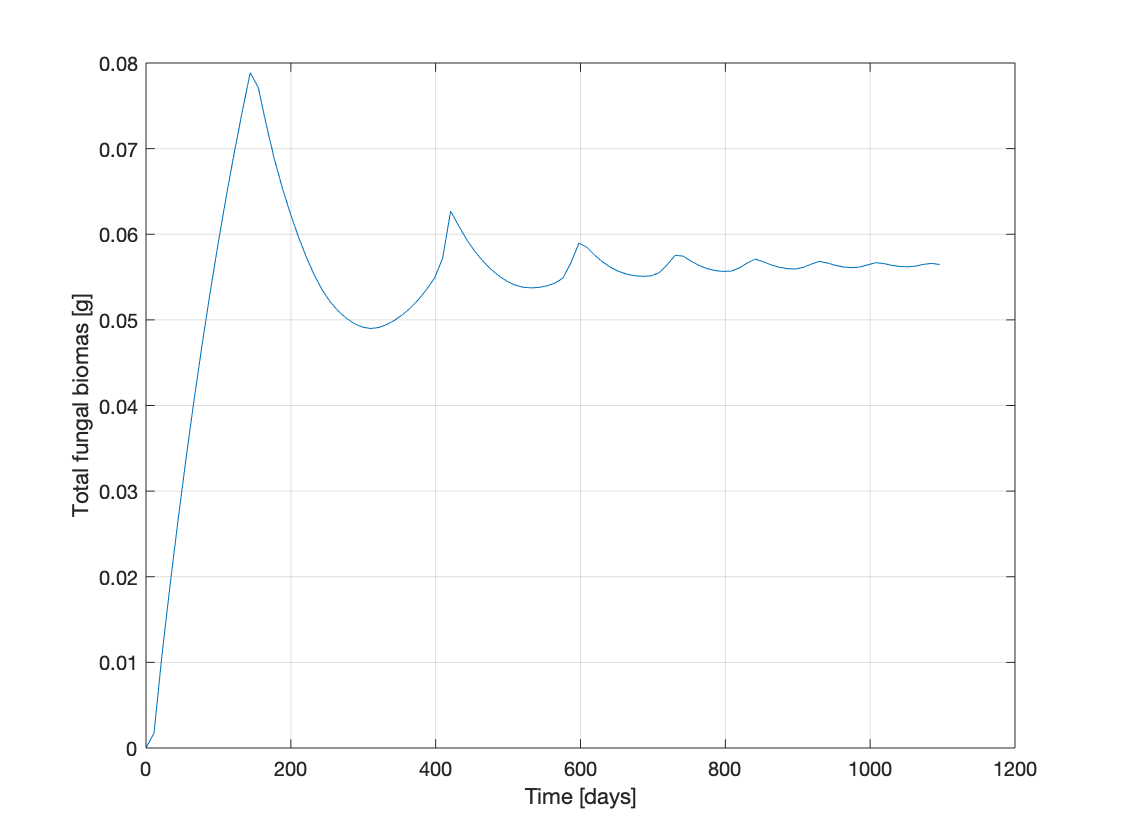
\includegraphics[width=\linewidth]{biomass_growth_no_Cterm.png}
%\captionof{figure}{Figure caption}
%\label{Fig 2.}
%\end{center}
%\begin{multicols}{2}

\subsection{Representative results}
We ran the coupled growth and decomposition model using parameters summarized in Table \ref{table3} to obtain a representative result. In the growth model, $\rho$ was found to exhibit travelling wave dispersion throughout space, as similarly shown in Mimura et al. (2000) and Edelstein (1982) \cite{Mimura2000, Edelstein1982}. As a consequence of only running the simulation for a timespan of three years, the decrease in carbon over time looks fairly linear, with slight fluctuations likely due to the fluctuating fungal biomass densities over time. 

In the first initial runs, no coupling term defining a limited nutrient availability was present in the growth equations. This eliminated the effects of decreasing concentration of carbon as the growth model assumed an abundance of nutrients was present. Under short time scales this could be a perfectly valid assumption, as short time scales tended to show little overall decrease in the concentration of holocellulose carbon. However the consequences seen from introducing this term in the growth equations become more apparent as longer time scales are considered. These effects can be seen in our results. The outcome for overall biomass of the communitty was mostly unaffected other than replacing decaying oscillations towards a steady state with a somewhat constantly increasing biomass overtime with a decaying slope. 

Overall, including the nutrient availability term in the growth equation captures more of the fundamental interaction that this paper is concerned with (that of decomposing wood and ground litter rather than free-growing fungi), so it remained present for further analysis.

\section{Analysis}

\subsection{Distribution of relative concentration of fungi}
The model allows us to adjust the relative concentrations of each fungi species being simulated. In the model, this is represented with a set of $0<c_{i}\leq 1$ such that $\sum c_{i} = 1$. Each one of these $c_{i}$ multiplies the rates of hyphal density increase and boundary/initial conditions in the growth model. With this metric, the relative concentrations of different fungi species are forced to satisfy the conditions $B_{i}/B_{tot}=c_{i}$ where $B_{i}$ is the biomass of the '$i$'th fungi species. This is an unrealistic constraint, as the relative concentrations of different fungal species should fluctuate with time as the different species of fungi grow at varying rates. But for the purpose of assessing the effect of biodiversity on the overall decomposition of the substraight, concentration fluctuation would add unneeded complexity to the analysis. \\
This analysis also considers the competitive rankings of the different fungi species \cite{Maynard2019}. The ranking-distribution coefficient, $a$ is then defined to be
\begin{equation} \label{eq}
a = \sum_{i=1}^{n} c_{i}*R_{i}
\end{equation}
Where $R_{i}$ s the competitive ranking for the '$i$'th fungi species. The ranking-distribution coefficient can be though of as a dot-product in $n$-dimensional space (where $n$ is the number of various fungi species being simulated). So $a$ will be highest when the $n$-dimensional vectors "line-up" in the sense that the distribution of fungi species is closest to the distribution of competitive rankings.\\
To study the effects of $a$ on the system overall, sample $c$ values had to be chosen. Due to a lack of literature results on simple, constant fungi distributions, arbitrary Gaussian distributions spread out over the different species of fungi were chosen. Because we are mainly concerned with the relation of any given distribution to the competitive rankings, the functions can be viewed as arbitrary or random distributions (because the ordering of fungal species in our Gaussian distribution has no physical meaning). The results of model runs using these various distributions is shown in (figure carbon-decrease-fungi-distribution). To assess the overall effectiveness of a single species distribution, the average carbon decrease over the whole interval was found via the equation $C_avg = \int (C_{0}-C)dt/(\delta t)$ where $C_{0}$ is our initial amount of carbon and $\delta t$ is the total time change over which the carbon decreases. The results of comparing this average carbon decomposed to the $a$ value for the species distribution in question is seen in (figure a-competative-distribution-coef-to-avg-Clost). Several interesting qualitative behaviors arise from the this comparison. Firstly, there is a clear smooth trend between $a$ and the average carbon decomposed up to approximately $a=0.65$. At this point the smooth trend completely vanishes and the data points appear to be randomly distributed in the area. We hypothesize that this critical value of $a$ could be representative of a bifurcation point; however further analysis on the dynamics of these coupled systems interacting would need to be done to investigate this hypothesis further. Additionally we notice that at this critical point, the average carbon decomposed tends to grow significantly. The physical interpretation of this critical point is deeply related to the effectiveness of the competitive rankings as they relate to a biologically diverse system. The results show that beyond a certain point, distributing the biodiversity more closely to the competitive rankings does not have any noticeable effect on the overall effectiveness of the system. \\
This leads to two possibilities beyond the critical point for the system. One possibility is that optimum biodiversity is based on more complex dynamics than the competitive rankings can assess. The other possibility is that the system behaves in a chaotic or random nature beyond this critical point and no clear metric of biodiversity could be correlated to the effectiveness of a given distribution.

\subsection{Environmental fluctuations}
Realistically, the external environment dictates environmental conditions of the system both in short time scales (year fluctuations for example) and long time scales. Due to the time scales of our model, the effects of very fast fluctuations (due to outside forces) on the scale of days are not considered as relative changes in the model's state have negligible changes on the order of a day. Thus we define our short term fluctuations to be roughly seasonal as this dictates the majority of local environmental variability. To study the effects of these short time scale fluctuations, we choose to implement an abstracted yearly moisture cycle, specifically that of the temperate forest environment. The cycle oscillates between the average yearly maximum and minimum values of $\psi$ twice a year, creating a rough yearly pattern of $\psi$ and thus $\nu$ for a given fungi from experimental data \cite{Zobel2001}\cite{Maynard2019}. Note that this moisture model is limited in assuming one period oscillation between a maximum and a minimum yearly, neglecting the reality of oscillating between local minimum in summer and winter and locate maximums in fall and spring. To incorporate this into the model, $\nu$ and $\psi$ were dynamically allocated over time based on the oscillatory behavior shown in (figure oscillating-psi-nu). Due to time limitations and scarce data on the parameters over these yearly oscillations, only two species of fungi were simulated. A comparison of their respective decomposition contributions with that of similar environmental conditions but static $\nu$ and $\psi$ is shown in (figure oscillating2nonoscillating-psi-contribution). There is no note-worthy new oscillatory motion seen in these results. There is also seen to be a slight increase in the effectiveness of both fungi in the oscillatory case. The interpretation of this increase can be that for time scales on the order of a year, the positives affect of increasing $\nu$ is greater than that of the negative affect of decreasing $\nu$ by the same amount. This would lead us to believe that faster oscillations of $\nu$ will generally have a positive net impact on the decomposition. The frequency limits of this principle would require further investigation. 


\subsection{$\nu$ vs Average Contribution to Substrate Decay} %avg_contr_nu_environment.fig
Using the decomposition model, average contribution to substrate decay and the tip elongation rate $\nu$ can be found for each fungal species for a given environmental configuration. Aside from indicating an expected positive correlation between $\nu$ and contribution, we find that in general, environments with a higher moisture potential lead to greater contributions overall and a greater contribution sensitivity to $\nu$ in our model. Our model agrees with the notion of water potential serving as an important limiting factor to the decomposition ability of individual fungi. This corroborates with various findings, that find soil moisture as a particularly influential environmental factor, influencing elongation through pressure gradients and testing of tolerance \cite{Maynard2019} \cite{Lustenhouwer2020}. %i think there may be a better citation, i am tired
%****In case linear regression added: The tropical rain forest environment, with a water potential of 0.76, lead to a }

\subsection{Total Carbon vs Time for Specific Environments} %direct_compare_decom_environmen.fig
Similarly, a sampling of different environmental parameters within the decomposition model demonstrates the decrease of total carbon in a fungal-waste system over time. Here, we see more moist soil environments lead to clearly more expedient rates of carbon total carbon decrease and reach total decomposition quicker in our model. Again in the model, the rain forest environment exceeds the other environmental profiles, effectively completing decomposition in under 1640 days (roughly 4.5 years.

\subsection{Average Contribution vs $\nu$ with Competitive Rankings} %avg_contr_nu_competative_rankings.fig  Maybe ask trevor to change colors or flip colors (final point(s) difficult to see
With one set of environmental parameters, we can gain insight into how different species of fungi potentially interact relative to each other. In addition to an expected lose positive correlation between $\nu$ and the average contribution of a given fungi, these is a lose correlation of higher fungi competitive ranking with greater $\nu$ and greater average contribution. This suggests that the fungi that are more 'active' in our model, with the largest growth rates and proportions, are also the most competitive. Competitive ranking has a higher correlation with $/nu$, indicating that in our model growth rate may be more significant than proportion when it comes to competitive circumstances. This aligns with established trends of the primary 2 fungal niches \cite{Maynard2019}.

\section{Limitations}
\subsection{Growth Coupling}
The coupling between our growth model and our decomposition kinetics model was scarsely found in literature. Instead, literature would in some cases adopt a simpler mechanism to describe fungi growth to match decomposition kinetics of equal complexity to our model, or would in other cases implement a more complex mechanism for fungi nutrient uptake while neglecting much of the complexity from interactions between fungi and with the larger environment. This resulted in a lack of applicable parameters from literature to choose from for our coupled model, for which we decided either to pull parameter values from simpler models described above or to empirically derive our parameters by fitting the model output to other reasonable outputs (as was done with the parameter $G$). 

\subsection{Parameter Choices and Enzyme Concentration}
In our comparison of different methods for coupling the growth equation to the decomposition kinetics, there are some unrealistic disagreements between the early behavior of each growth model; mainly that of a slight increase in the first maximum biomass reached by the carbon limiting growth model. Expected behavior would exhibit less biomass gained over time when the nutrient level is limited. This result is likely a consequence of bad parameter choices derived with imperfect methods described above or a failure to incorporate a more realistic relationship between the decomposed carbon pool and available carbon pool from which the fungi supplement their own nutrient supply.

The Michaelis-Menten dynamics we implemented often considers enzyme concentration to be proportional to the maximum rate of the reaction. Taking this concentration to be proportional to total fungal biomass in some set region of space does not account for the concentration of enzymes becoming saturated as the fungi spread farther out through space. A more realistic incorporation of this idea into the model would need to address the geometric complexities involved in examining only one region of a much larger fungi growth. Even further unpackaging of these dynamics would account for fungal growth into areas that do not have physical access to the carbon being decomposed. At this point, a simplified one-dimensional growth model would not suffice.

The effect of considering biomass proportional to concentration would be seen in the longer term behavior of the model, as the fungi growth becomes limited. We may expect to see more complex dynamics transitioning between the "unbounded" fungi growth and the steady-state behavior of fungi growth. Thus, the largest area of error for our results due to this assumption is likely in the area of time transitioning unbounded growth and steady-state behavior.

\subsection{Direct Interactions}

It was observed in literature that there are direct interactions between fungi growing in the same environment by various mechanisms (NEED CITATION). Our model ignored the effects of these direct interactions and instead focused on indirect interactions via competition for the same nutrients source. The effects of fungi's mechanisms of sabotage via physical means is typically taken to be negligible and the dynamics of such interactions are likely too complicated to consider. However, the effect of space-limitation would likely cause there to be non-negligible limitations on fungal growth due to others obstructing their path or due to total lack of available space. Essentially, our simulation considered fungi competing for food, when in reality, they compete for food and space. In considering these effects, care must be taken to the space of consideration and the limitations of that space. Further review would need to be done to assess the limitations of various spaces, but because we are considering fungi in open ground liter without any obvious obstructions to their growth, spacial limitations on the fungi growth may be considered negligible. This assumption would not apply in the case of geometric isolation of a particular fungi but the geometric access of particular fungi to the substraight is another complexity that would need to be addressed in a higher-dimensional growth model. 


%\begin{ColumnFigure}
%	\centering
%	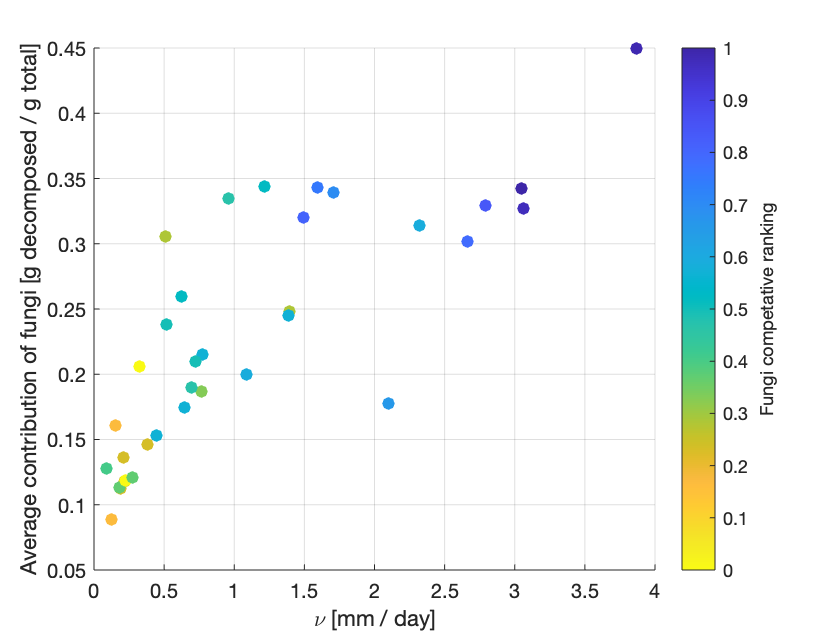
\includegraphics[width=\linewidth]{avg_contr_nu_competative_rankings.png}
%	\captionof{figure}{my caption of the figure}
%\end{ColumnFigure}
\end{multicols}
\newpage
\appendix
\section{Model Parameters}

Here are the model parameters for the coupled growth and decomposition model for Armillaria gallica located at 30.465247 degrees latitude and -89.040298 degree longitude secreting cellobiohydrolase (Cel7A) to decompose hardwood holocellulose \cite{Maynard2019, Kari2014}:

\begin{savenotes}
	\begin{table}[ht]
		\begin{center}
			\begin{tabular}{|c c c c c|} 
				\hline
				Parameter & Symbol & Value & Units & Source and Specification \\
				\hline\hline
				Half-Saturation constant \footnote{Also called Michaelis Constant.} & $K_e$ & 7 & $\frac{g_{enzyme}}{L_{litter}} $ & \cite{Kari2014} Enzyme \\ 
				\hline
				Holocellulose carbon \footnote{We assume that all carbon compounds excluding lignin are holocellulose.} & $1-LCI \footnote{Where LCI is the lignocellulose index.}$  & 0.709 & N/A & \cite{Segato2014} \\ %confirm unitless
				\hline
				Hyphal tip elongation rate& $\nu$& 0.250 & $\frac{mm}{day}$ & \cite{Maynard2019} Species, $\psi$, T\\
				\hline
				Temperature & T & 25 & $^{\circ}C$ &\cite{Maynard2019} Specie's habitat\\
				\hline
				Water potential & $\psi$ & -0.5 & MPa &\cite{Maynard2019}\\
				\hline
				Enzyme biomass ratio \footnote{Proportion of specific enzyme biomass to total enzyme biomass.} & r & 0.437 & $\frac{g}{g}$ &\cite{Maynard2019} Species\\
				\hline
				Hyphal death rate& $\gamma_1$ & 0.15 & $day^{-1}$ &\cite{Schnepf2008}\\
				\hline
				Anastomosis coefficent & $\mu$ & 0.3 & $\frac{mm}{day}$ &\cite{Lyn2016}\\ % Trevor sussed on units
				\hline
				Branching rate & $\alpha_1$ & 1.2372 & $day^{-1}$ &\cite{Du2019}\\
				\hline
				Intercept of $S_M$ function \footnote{The intercept of soil moisture effect on decay rate.}& $\alpha_2$ & 0.311 & N/A &\cite{Moorhead1991}\\
				\hline
				Slope of $S_M$ function & $\lambda$ & 0.345 & $N/A$ &\cite{Moorhead1991}\\ % units? might be MPa^{-1}, but comes out of log?
				\hline
				Soil moisture coefficient & $S_M$ & 0.4149 & N/A &\cite{Moorhead1991} $\psi$\\ % mention equation later in paper
				\hline
				Soil temperature coefficient & $S_T$ & 1 & N/A &\cite{Moorhead1991} T\\
				\hline
				Rate of Increase & $Q$ & 2.5 & $^{\circ}C$ &\cite{Moorhead1991} T\\
				\hline
				Rate constant \footnote{Proportionality constant between maximum rate of decomposition and enzyme biomass.} & G & 10 & $g*mm^{-1}*day{-1}$ &\cite{Lustenhouwer2020}\footnote{Emprically derived.}\\  %value TBD, empirically derived, Trevor will justify
				\hline
			\end{tabular}
		\vspace*{-3ex}
		\captionof{table}{Model Parameters}\label{table3}
		\end{center}
	\end{table}
\end{savenotes}


\section{Appendix Tables}

\begin{table}[H]
	\begin{center}
		\begin{tabular}{|c c c|} 
			\hline
			Biome/ Environment & Average Annual Temperature [$^{\circ}C$] & Selected Value [$^{\circ}C$]\\ [0.5ex] 
			\hline\hline
			Dessert (Arid) & 10 to 20 \cite{Davey2007} & 15 \\ 
			\hline
			Grasslands/shrublands (Semi-Arid) & 15.3 \cite{Pelaez1994} & 15.3 \\
			\hline
			Temperate Forest & -1.42 to 26.39 \cite{Zaz2019} & 12.49 \\
			\hline
			Boreal Forest (Arboreal)& -1.42 to 26.39 \cite{Zaz2019} & 12.49 \\
			\hline
			Tropical Rain Forest & 23 to 32 \cite{Paton2019} &27.5 \\
			\hline
		\end{tabular}
	\vspace*{-3ex}
	\captionof{table}{Environment Temperature Data}\label{table6}
	\end{center}
\end{table}



%NEED TO EDIT TABLE WITH FOOTNOTES TO FIT (put spec envs?)
%For himalayas, consider putting all values as footnotes
\begin{savenotes}
	\begin{table}[H]
		\begin{center}
			\begin{adjustbox}{width=1\textwidth}
			\begin{tabular}{|c c c|} 
				\hline
				Biome/ Environment & Water Potential Range [MPa] & Selected Value [MPa] \\ [0.5ex] 
				\hline\hline
				Dessert (Arid) & -4.0 to -5.0 MPa \cite{Nilsen1983} & -4.5 MPa \\ 
				\hline
				Grasslands/shrublands (Semi-Arid) & -1.4 to -5.0 \footnote{Measurements taken November through January at 100 cm soil depth.} \cite{Pelaez1994} & -3.2 MPa\\
				\hline
				Temperate Forest & -0.44 (Fall), -1.19 (Winter), -0.58 (Spring), & -1.09 MPa\\
				&-1.42 (Early Summer), -1.81 (Summer) \cite{Zobel2001}&\\
				\hline
				Boreal Forest (Arboreal) & -0.83 (Fall), -1.20 (Winter), -0.55 (Spring),& -1.51 MPa\\
				&-1.61 (Early Summer), -3.36 (Summer) \cite{Zobel2001} &\\
				\hline
				Tropical Rain Forest & -1.57 MPa to 0.00 MPa \cite{Kupers2019} & -0.79 \\
				\hline
			\end{tabular}
			\end{adjustbox}
		\vspace*{-3ex}
		\captionof{table}{Environment Water Potential Data}\label{table4}
		\end{center}
	\end{table}
\end{savenotes}

\begin{savenotes}
	\begin{table}[H]
		\begin{center}
			\begin{adjustbox}{width=1\textwidth}
			\begin{tabular}{|c c c c c|} 
				\hline
				Parameter & Symbol & Value & Units & Source and Specification \\
				\hline\hline
				Half-Saturation constants \footnote{Also called Michaelis Constant.} & $K_e$ & - & mM &  Enzyme \\ 
				& $K_e$ - Phenol oxidase & 0.89 & mM &  \cite{Davidson2012}\\
				& $K_e$ - Phosphatase & 0.94 & mM &  \cite{Nannipieri2011}\\
				& $K_e$ - Peroxidase & 0.7475 & mM &  \cite{Chance1943}\\
				& $K_e$ - Cellobiohydrolase & 13.90 & mM &  \cite{Razavi2015}\\
				\hline
				Hyphal tip elongation rate& $\nu(T,\psi)$& Various & $\frac{mm}{day}$ & \cite{Maynard2019} Species, $\psi$, T\\
				\hline
				Soil moisture coefficient & $S_M$ & $S_M = \alpha_2 -\lambda \log_{10}(-\psi)$ & N/A &\cite{Moorhead1991} $\psi$\\ % mention equation later in paper
				\hline
				Soil temperature coefficient & $S_T$ & $\log_{10}(S_T) = \frac{T-25}{10}\log_{10}(Q)$ & N/A &\cite{Moorhead1991} T\\ 
				\hline
			\end{tabular}
			\end{adjustbox}
		\vspace*{-3ex}
		\captionof{table}{Environmental \& Parameter Table}\label{table5}
		\end{center}
	\end{table}
\end{savenotes}

\section{Appendix Figures}

Figures here

%\end{multicols}
\newpage
\printbibliography
\end{document}